\documentclass[11pt]{article}
\usepackage[T1]{fontenc}
\usepackage[utf8]{inputenc}
\usepackage{lmodern}
\usepackage[margin=1in]{geometry}
\usepackage{microtype}
\usepackage{amsmath}
\usepackage{booktabs}
\usepackage{tabularx}
\usepackage{xcolor}
\usepackage{listings}
\usepackage{tikz}
\usetikzlibrary{arrows.meta,positioning,calc}
\usepackage{pgfplots}
\pgfplotsset{compat=1.18}
\usepackage[numbers,sort&compress]{natbib}
\usepackage[hidelinks]{hyperref}
\usepackage{caption}
\captionsetup{font=small,labelfont=bf}

\definecolor{broken}{HTML}{C0504D}
\definecolor{fixed}{HTML}{4E9A4E}
\definecolor{accent}{HTML}{2F6FDB}
\definecolor{muted}{HTML}{A8A8A0}
\definecolor{edge}{HTML}{8A8A82}

\lstdefinelanguage{PHPx}{language=PHP,morekeywords={public,function,self,null,false,is_countable,count}}
\lstset{language=PHPx,basicstyle=\ttfamily\footnotesize,columns=fullflexible,keepspaces=true,
  commentstyle=\color{black!55}\itshape,keywordstyle=\bfseries,frame=single,framerule=0.3pt,
  rulecolor=\color{black!30},xleftmargin=4pt,xrightmargin=4pt,breaklines=true,showstringspaces=false}

\newcommand{\code}[1]{\texttt{#1}}
\emergencystretch=2em

\title{Tools, Not Prompts: Revisiting LLM-Based Legacy PHP Modernization with an Agent Harness}
\author{Ianiv Schweber - Just a random guy on the Internet}
\date{November 2, 2026}

\begin{document}
\maketitle

\begin{abstract}
A recent study evaluated five large language models (LLMs) on modernizing 100 WordPress 4.0 PHP files to PHP 8.3.
Given one prompt per file and no tools, tests, or runtime feedback, every model ended with fewer behaviorally compatible files than leaving the code unchanged (83 of 100).
The study scopes this finding to the first answer of a single-file workflow, and it anticipates both newer models and execution feedback.
Its headline is nonetheless easy to repeat as evidence that LLMs cannot produce working migrations.
We test that broader reading, not the authors' scoped claim, with the study's own released harness (630 hidden PHPUnit checks and Rector's PHP-version rules) and Claude Opus 5.5.
Under the study's single-shot protocol and limits, Opus 5.5 produces 93 compatible files and breaks one originally compatible file.
As a coding agent with PHP 8.3, the file's checks, a linter, and Rector, scored on a pristine copy of the harness, it produces 99 compatible files with zero regressions.
Both conditions exceed the unchanged code significantly (exact McNemar, Holm-adjusted $p \le 0.025$); the difference between them is not significant on a single run.
The agent condition implements the staged, execution-feedback workflow that the original study recommends, and it has access to the very checks that score it, so it measures what a developer with a test suite can achieve.
The one file the agent does not pass is blocked by a defect in that file's test environment.
We validate our harness by reproducing the published baseline, the Sonnet 4 and Rector results, and, with a reconstructed rule mapping, the study's necessity breakdown and sensitivity analyses.
\end{abstract}

\section{Introduction}

Much of the web still runs PHP that was written for PHP 5.
PHP 7 and 8 removed or redefined many of the constructs that code depends on: \code{each()}, \code{create\_function()}, curly-brace string offsets, PHP 4-style constructors, and lenient handling of \code{null} and non-countable values.
Moving such code to a supported runtime is costly, repetitive, and easy to get subtly wrong, which makes it a natural target for automation.

The study we revisit~\cite{mahmud2026modernization} asks whether LLMs can do this work safely.
It samples 100 files from WordPress 4.0 and asks five models to migrate each file to PHP 8.3 in a single prompt.
It then scores the outputs with 630 hidden PHPUnit checks and with Rector's PHP-version rules.
Its headline finding is negative.
Under PHP 8.3, 83 of the 100 unmodified files are behaviorally compatible, while the best model reaches 59.
The rule-based tool Rector reaches 82.

That finding is accurate for the condition the study measures, and the study is careful to say so.
It evaluates ``the first answer, not an agent's result after iterating on errors'' (\S I).
It notes that ``newer models may avoid specific errors, but the evaluation design applies unchanged'' (\S V).
And it recommends treating the first answer as a draft: a staged workflow of lint, load with dependencies, then check behavior, after which ``execution feedback could then drive repair'' (\S V).
A headline such as ``every evaluated LLM left fewer working files than it started with'' is nonetheless easy to repeat without these qualifications, as evidence that LLMs cannot migrate legacy code.
Within days of posting, one article headlined the study ``AI Legacy Code Modernization Breaks More Working Code Than It Fixes''~\cite{cava2026generativelabs}, although its body does note that each model got ``one file, one prompt and no chance to run its own output.''
This paper tests that popular reading, not the authors' claim.

The popular reading depends on the two things the study deliberately sets aside.
The first is model generation.
The models evaluated in~\cite{mahmud2026modernization} were released between December 2024 (Llama 3.3 70B~\cite{meta2024llama33}) and September 2025 (GPT-5 Codex~\cite{openai2025codex}).
Claude Sonnet 4 dates from May 2025~\cite{anthropic2025claude4}, and both Gemini 2.5 models became generally available in June 2025~\cite{google2025gemini25}.
The study's tool documentation was accessed in August 2026 and the paper was posted at the end of October 2026, so the models were roughly one to two years old when it appeared.
The second is execution feedback.
In the study, a model sees one file and nothing else, and it never runs, lints, or tests its output, whereas coding agents iterate against an interpreter and a test suite.
We therefore ask how much of the gap a newer model closes under the identical protocol, and what the study's own recommended workflow achieves.

We answer them with the study's own artifacts. We pose three research questions:
\begin{itemize}
  \item \textbf{RQ1 (Reproduction).} Can the released harness be run independently and reproduce the published baseline and model results?
  \item \textbf{RQ2 (Model).} Under the identical single-shot protocol, how does a current frontier model (Claude Opus 5.5) compare with the models in the original study and with the unchanged code?
  \item \textbf{RQ3 (Harness).} When the same model runs as a coding agent with an interpreter, the file's checks, a linter, and Rector (the staged workflow recommended in~\cite{mahmud2026modernization}), how close does it come to a complete and behavior-preserving migration?
\end{itemize}

Our contributions are:
\begin{enumerate}
  \item An independent reproduction of the study's evaluation on macOS with PHP 8.3 in a Linux VM. It matches the no-change baseline check for check and the published Sonnet 4 and Rector results exactly. With a reconstructed rule-to-necessity mapping it also reproduces the study's resolution-by-necessity table and its sensitivity analyses.
  \item A single-shot replication with Opus 5.5 that keeps the study's prompt, extractor, and limits. Opus 5.5 alone exceeds the no-change baseline (93 vs.\ 83 compatible files).
  \item An agent harness, scored on a pristine copy of the harness, that reaches 99 of 100 compatible files with zero regressions. We trace the remaining file to a defect in its test environment.
  \item A released replication package with all outputs, scores, each agent session's final report and run statistics, the re-analysis, and a contamination check against later WordPress releases.
\end{enumerate}

\section{Background and Related Work}

\paragraph{Rule-based migration.}
Rector~\cite{rector} rewrites PHP abstract syntax trees using rule sets keyed to language versions, such as \code{UP\_TO\_PHP\_83}.
Its rules are local and mechanical, so they rarely change behavior that already works.
For the same reason, they cannot repair failures that depend on semantics: a \code{count()} on \code{null}, which now throws, or a comparison whose result changed in PHP 8.
The original study uses Rector both as a baseline and as the source of its legacy-pattern metric.

\paragraph{Evaluating behavior, not text.}
TransCoder~\cite{roziere2020transcoder}, an unsupervised neural translator between C++, Java, and Python, introduced \emph{computational accuracy}: a translation counts as correct only if it produces the reference outputs on unit tests.
Its motivation is the gap that the hidden checks of~\cite{mahmud2026modernization} also address.
Only 3.1\% of TransCoder's C++-to-Java translations matched the reference text, yet 60.9\% passed the tests.
TransCoder also used the tests to choose among beam-search candidates, which raised computational accuracy by up to 33.7 points (Java to Python).
Choosing by execution is the simplest form of the feedback our agent condition provides.

\paragraph{LLMs silently change behavior when translating.}
Pan et al.~\cite{pan2024lost} found that 2.1\% to 47.3\% of LLM code translations were correct, depending on the model.
Most failed translations (77.8\%) did not compile, but 13.4\% of them compiled and ran yet failed tests.
That silent change of behavior is the failure mode the hidden checks of~\cite{mahmud2026modernization} detect.
Re-prompting with the error output, plus a failing input and expected output for test failures, raised GPT-4's success rate by 12.33\% after one round and the four repaired models' by 5.5\% on average, although some repairs turned one kind of bug into another.
Our preservation metric tracks this risk: repair in a loop must not cost regressions.

\paragraph{Execution feedback, not iteration, drives the gain.}
Self-debugging~\cite{chen2024selfdebug} lets a model revise its code from feedback over up to 10 turns.
On C++-to-Python translation it raised Codex from 80.4\% to 92.5\% when the feedback included unit-test results and the model's own explanation of its code, but only to 83.9\% when the model could explain or trace its code without executing the tests.
This split between generation and execution feedback mirrors our RQ2 and RQ3 at function scale.

\paragraph{Agents on repository-scale tasks.}
SWE-bench~\cite{jimenez2024swebench} judges a patch by tests that must go from failing to passing and tests that must keep passing.
These are the same repair and preservation criteria that~\cite{mahmud2026modernization} uses.
Its baselines generate a patch in one pass from retrieved files, and the best resolved 1.96\% of issues.
With the same model (GPT-4 Turbo), SWE-agent~\cite{yang2024sweagent} raised the resolve rate on SWE-bench Lite from 2.67\% for that single-pass baseline to 18.0\%, by letting the model navigate the repository, edit files, and run code.
Its ablations credit a linter that rejects syntactically invalid edits with 3.0 of those points.
Our agent's \code{tools/lint} serves the same role.

\paragraph{Evaluation condition as a variable.}
Our study treats the presence of execution feedback as an experimental factor, separate from the model.
To isolate the model's contribution we hold the prompt, file, and scoring fixed (RQ2).
We then add the tool loop with the model held fixed (RQ3).

\section{The Original Study}

\paragraph{Dataset.}
The study~\cite{mahmud2026modernization} draws on WordPress 4.0's 482 PHP files.
It keeps the 397 that have Rector findings and selects 100 by a deterministic, stratified procedure that covers all rule types.
By size, 31 files have at most 200 lines, 31 have 201--500, 26 have 501--1,000, and 12 exceed 1,000 lines.
Together they total 54,321 lines.

\paragraph{Hidden checks.}
The study defines 630 PHPUnit checks: 109 reachability checks, 441 output or state checks, and 80 semantic-fingerprint checks.
Each test file targets one subject.
It runs the subject in a sandbox built from the WordPress 4.0 tree plus per-file stubs, under PHP 8.3 with \code{E\_ALL}, and it counts deprecation notices as failures.
Unmodified, the files pass 531 checks.
The harness report in the study's replication package~\cite{mahmud2026package} attributes the 99 failures to removed or changed PHP features: 59 parse errors, 21 output mismatches, 8 undefined symbols, 6 type or signature errors, and 5 fatal runtime errors.

\paragraph{Metrics.}
For a migrated variant, each check falls into one of four transitions relative to the original: preserved pass, regression, repair, or unrepaired failure.
The study reports:
\begin{itemize}
  \item \textbf{Compatible files:} files whose checks all pass.
  \item \textbf{Preservation:} preserved passes $\div$ 531, the original passes that still pass.
  \item \textbf{Repair:} repairs $\div$ 99, the original failures that now pass.
  \item \textbf{Legacy-pattern resolution:} Rector \code{Php*} findings in the original that no longer fire after migration. A finding is a (file, rule type) pair; there are 511 across 44 rule types. Rector runs on each file in isolation, and unparseable output resolves nothing.
\end{itemize}

\paragraph{Necessity.}
The study groups Rector's findings by what happens if the construct is left unchanged under PHP 8.3.
\emph{Required} constructs fail or change behavior (for example, curly-brace string offsets or PHP 4-style constructors), \emph{deprecated} ones run but raise notices, and \emph{optional} ones remain valid.
Only 37 of the 511 findings are required, against 85 deprecated and 389 optional, and optional changes make up 82--87\% of what each model resolves.
The study's central observation is that most broken files needed no required change: the LLMs break 36--60\% of the compatible files that contain no required finding.
In its words, ``resolution measures what changed, not whether it should have.''

\paragraph{Condition.}
Each model receives a fixed prompt that asks a senior PHP developer to migrate the file to PHP 8.3 while preserving functional equivalence, followed by the full file.
Temperature is 0.2, except for GPT-5 Codex, whose API does not expose it; reasoning and thinking settings stay at provider defaults.
Requests allow up to 64,000 output tokens and 600 seconds.
The study keeps the first complete response, regenerating incomplete ones, and extracts code between \code{// MIGRATION\_START} and \code{// MIGRATION\_END} markers.
The model sees no other files, tests, or errors.

\paragraph{Statistics and sensitivity.}
File-level compatibility is compared with two-sided exact McNemar tests under Holm--Bonferroni correction, and effect sizes are paired differences in compatible files with 95\% percentile bootstrap intervals (10,000 file resamples).
Two sensitivity analyses recount compatible files without the 80 fingerprint checks and with a lint fallback, which substitutes the original for any output that \code{php -l} rejects.

\paragraph{Reported results.}
Every LLM falls below the unchanged code on compatible files: Sonnet 4 reaches 59, GPT-5 Codex 58, Gemini 2.5 Pro 55, Gemini 2.5 Flash 50, and Llama 3.3 70B 33, against Rector's 82.
With the lint fallback the best LLM, GPT-5 Codex, reaches 69 (Sonnet 4: 67), still below the unchanged code.
The study does not score Rector's own resolution, which would be circular.
The full figures appear alongside ours in Table~\ref{tab:main}.

\section{Methodology}

\subsection{Environment and harness reproduction}

We download the study's replication package~\cite{mahmud2026package} and run it unchanged except for the runner.
The package's PowerShell runner sets three environment variables and calls PHPUnit, so we port it to a 10-line bash script.
PHP runs in a Linux VM under Apple's \code{container} (v1.6.1, Virtualization.framework) from the official \code{php:8.3-cli} image, which provides PHP 8.3.36.
It includes the bcmath, curl, dom, mbstring, pdo, simplexml, tokenizer, xml, and zip extensions, with \code{error\_reporting=E\_ALL}.
Tools come from the package's lock files: PHPUnit 9.6.34 and Rector 2.1.0.

We validate the reproduction three ways before running any model (RQ1):
\begin{enumerate}
  \item Run the unchanged originals and diff the per-check testdox output against the package's \code{OriginalTestResults.txt}.
  \item Re-score the package's archived Sonnet 4 outputs end to end and compare with the published summary.
  \item Run Rector on every original and count \code{Php*} findings against the package's metadata.
\end{enumerate}

\subsection{Single-shot condition (RQ2)}

We reuse the study's prompt template verbatim, insert the full file, and extract code with a line-for-line port of its extractor.
Like the original, we read files as UTF-8 with undecodable bytes ignored.
Calls go to Claude Opus 5.5 through the Claude Code CLI in print mode, with every tool disabled, a one-line system prompt, no user or project settings, and a 64,000-token output cap.
As in~\cite{mahmud2026modernization}, we keep the first complete response and regenerate incomplete ones, up to three attempts.

Two details differ from a raw API call.
The CLI does not expose temperature, so sampling uses the default, as the original study did for GPT-5 Codex, whose API does not expose it either.
Opus 5.5 also uses adaptive extended thinking by default, which we leave on: on file 004 it spent 3,786 thinking tokens.

The CLI's output cap applies per assistant turn, and the CLI continues a response that reaches it.
One response did so.
For file 014 (\code{module.tag.id3v2.php}, 134\,KB, the largest subject), the model used 84,406 output tokens (18,611 of them thinking) over two turns and 619\,s.
That exceeds the study's limits of 64,000 tokens and 600 seconds.
Opus 5.5's migrated code alone is about 65,800 tokens, so its response could not fit within those limits, and under the original protocol this file would have had no complete Opus response (Sonnet 4's shorter output for this file did fit, and passes all six checks).
We therefore count file 014 as failed in our primary, \emph{strict} single-shot result (93 compatible files), and we report the response as delivered (94) alongside it.
No other response exceeded 62,554 output tokens or 417\,s, or needed a second turn.

\subsection{Agent condition (RQ3)}

Each file gets its own workspace.
It is a copy-on-write clone of the harness with every archived model output, result file, and report removed, so the agent cannot see how other models did.
The subject directory starts as a copy of the originals.
The agent may edit exactly one file, the migrated copy of its subject.

Five tools run inside the PHP 8.3 VM:
\begin{itemize}
  \item \code{tools/test} runs the file's checks against the migrated copy.
  \item \code{tools/test-original} runs the same checks against the original.
  \item \code{tools/lint} runs \code{php -l}.
  \item \code{tools/rector} lists the remaining \code{Php*} findings, with the diff Rector would apply.
  \item \code{tools/php} runs the PHP CLI for scratch scripts.
\end{itemize}

The agent can read the checks, the stubs, and the full WordPress 4.0 tree.
Its instructions restate the study's goal of migrating to PHP 8.3 while preserving observable behavior.
They add a definition of done: every check passes, no Rector finding remains unless applying it would change behavior or call compatibility (with a reason for each one kept), and lint is clean.
They forbid edits outside the target, special-casing test inputs, detecting the test environment, and deleting uncovered functionality.

The agent is Claude Code (v2.1.316) in headless mode with model \code{claude-opus-5-5} and default effort.
It runs in \code{dontAsk} permission mode, with an allowlist of file tools, the five tools, and read-only shell commands.
Web access, \code{curl}, and \code{wget} are denied, and user settings, hooks, and MCP servers are not loaded.
Each file gets one session with no turn limit, and six sessions run in parallel.

The task prompt names the target file, its original, and its test file.
It was also meant to give the file's path in the WordPress tree, but a lookup bug left that path blank in 85 of the 100 prompts (``It is the WordPress file \code{``}.'').
The lookup matched \code{config/file-map.php} keys exactly, and from file 013 on most keys carry a \code{.php} suffix that our subject IDs do not.
The 15 prompts with a path are exactly the 15 files whose key has no suffix (001--012, 014, 016, and 030).
The omission removes information rather than adding any, and every agent still had the target, its tests, and the full tree.

\subsection{Run history}
\label{sec:runs}

We report every launch, including those that produced no model output.
\begin{itemize}
  \item \textbf{Agent, file 004.} Run first, alone, as a pilot. Its first launch hung while cloning the workspace, because of 21\,GB of leftover test sandboxes, and was killed before the agent started. The second launch is the shipped session. The task prompt did not change afterwards.
  \item \textbf{Agent, batch.} The other 99 files ran in one logged batch. Files 003 and 008 failed before their agents started, because the path lookup also matched example comments in \code{file-map.php} and broke prompt construction. We anchored the lookup and ran those two once more. No file was run more than once with a model session, and no completed session was discarded.
  \item \textbf{Single-shot.} A pilot call on file 004 was kept as that file's response. The batch started with 4 parallel calls and was restarted with 8, keeping every completed response. File 062's worker crashed on an encoding error before making any call, and we fixed it by reading files exactly as the original does (UTF-8, undecodable bytes ignored). File 014's first two responses were discarded because our extractor read only the last turn of each multi-turn response, which we then fixed. All three 014 responses spanned two turns and ran for about ten minutes, beyond the study's limits, which is why the strict result counts the file as failed.
\end{itemize}

\subsection{Scoring}

Both conditions are scored by the same pipeline.
It builds a fresh copy of the released harness, copies in only each run's migrated target files, and runs all checks.
It then runs Rector on each migrated file in its own directory, matching the study's single-file isolation.
Because tests, stubs, and configuration come from the pristine copy, an agent's edits outside its target cannot affect its score.
After each session we diffed the agent's tests, configuration, and other subject files against the pristine harness.
After the runs we extended that check to every file in each retained workspace (the WordPress tree, \code{vendor/}, \code{phpunit.xml}, Composer files, tests, configuration, originals, and the other subjects), excluding only the target, \code{scratch/}, \code{tools/}, and \code{build/}.
We count the 630 checks of the study, which, like the study, excludes the package's setup smoke test (Section~\ref{sec:rq1}).

\begin{figure}[t]
\centering
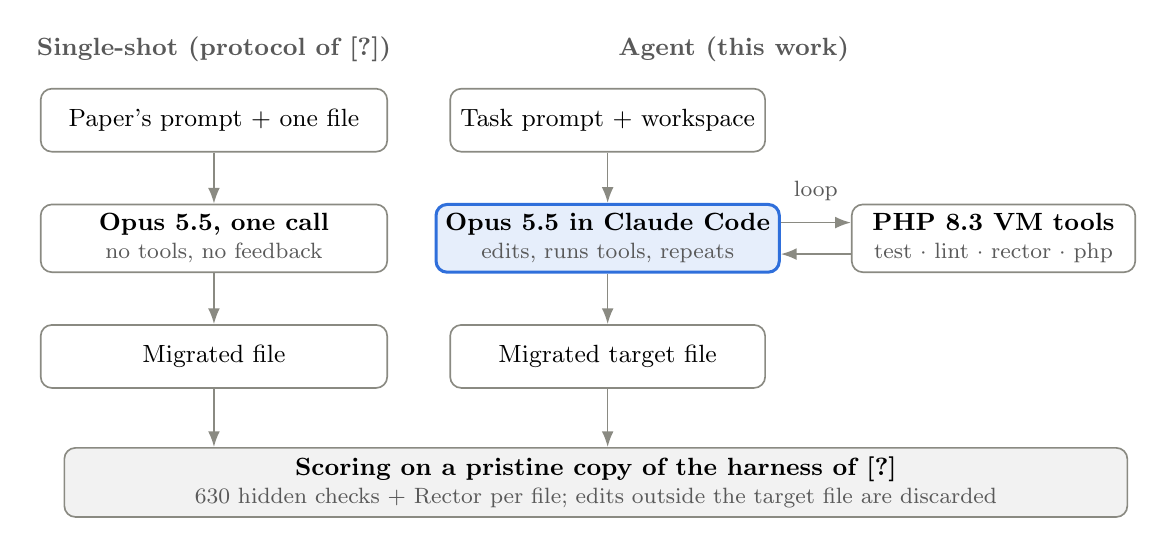
\begin{tikzpicture}[font=\small,
  box/.style={draw=edge,rounded corners=4pt,minimum height=8mm,align=center,line width=0.6pt},
  hot/.style={box,draw=accent,fill=accent!12,line width=1.1pt},
  arr/.style={-{Latex[length=2mm]},draw=edge,line width=0.6pt}]
  \node[font=\small\bfseries,text=black!65] at (0,0.9) {Single-shot (protocol of~\cite{mahmud2026modernization})};
  \node[font=\small\bfseries,text=black!65] at (6.6,0.9) {Agent (this work)};
  \node[box,minimum width=44mm] (a1) at (0,0) {Paper's prompt + one file};
  \node[box,minimum width=44mm] (a2) at (0,-1.5) {\textbf{Opus 5.5, one call}\\[-1pt]{\footnotesize\color{black!65}no tools, no feedback}};
  \node[box,minimum width=44mm] (a3) at (0,-3.0) {Migrated file};
  \node[box,minimum width=40mm] (b1) at (5.0,0) {Task prompt + workspace};
  \node[hot,minimum width=40mm] (b2) at (5.0,-1.5) {\textbf{Opus 5.5 in Claude Code}\\[-1pt]{\footnotesize\color{black!65}edits, runs tools, repeats}};
  \node[box,minimum width=40mm] (b3) at (5.0,-3.0) {Migrated target file};
  \node[box,minimum width=36mm] (t) at (9.9,-1.5) {\textbf{PHP 8.3 VM tools}\\[-1pt]{\footnotesize\color{black!65}test $\cdot$ lint $\cdot$ rector $\cdot$ php}};
  \node[box,fill=black!5,minimum width=135mm] (s) at (4.85,-4.6) {\textbf{Scoring on a pristine copy of the harness of~\cite{mahmud2026modernization}}\\[-1pt]{\footnotesize\color{black!65}630 hidden checks + Rector per file; edits outside the target file are discarded}};
  \draw[arr] (a1) -- (a2); \draw[arr] (a2) -- (a3); \draw[arr] (b1) -- (b2); \draw[arr] (b2) -- (b3);
  \draw[arr] ([yshift=2mm]b2.east) -- ([yshift=2mm]t.west);
  \draw[arr] ([yshift=-2mm]t.west) -- ([yshift=-2mm]b2.east);
  \node[font=\footnotesize,text=black!65] at ($(b2.east)!0.5!(t.west)+(0,0.6)$) {loop};
  \draw[arr] (a3) -- (a3 |- s.north); \draw[arr] (b3) -- (b3 |- s.north);
\end{tikzpicture}
\caption{The two experimental conditions and the shared scoring pipeline. Both receive the same file and are scored by the same pipeline; only the agent can run code against the checks before submitting.}
\label{fig:method}
\end{figure}

\section{Results}

\subsection{RQ1: The harness reproduces the published results}
\label{sec:rq1}

The reproduction matches the study wherever both can be compared (Table~\ref{tab:repro}).

\begin{table}[t]
\centering\small
\caption{Reproduction checks against the released package.}
\label{tab:repro}
\begin{tabularx}{\linewidth}{>{\raggedright\arraybackslash}X >{\raggedright\arraybackslash}p{47mm} >{\raggedright\arraybackslash}p{44mm}}
\toprule
Check & Published & Reproduced \\
\midrule
Originals: per-check testdox outcome & \code{OriginalTestResults.txt} & identical, 631 of 631 lines \\
Originals: checks passed & 531 of 630 (paper text) & 532 of 631 (package); 531 of 630 without the smoke test \\
Originals: compatible files & 83 & 83 \\
Sonnet 4 archived outputs: per-check testdox & package \code{testdox.txt} & identical \\
Sonnet 4: compatible / preservation / repair & 59 / 76.3\% / 68.7\% & 59 / 76.3\% / 68.7\% \\
Sonnet 4: Rector findings resolved & 272 & 272 \\
Rector outputs: compatible / checks / regressions / repairs & 82 / 581 / 12 / 62 & 82 / 581 / 12 / 62 \\
Rector \code{Php*} findings on originals & 511 & 511 (per-file isolation); 574 (whole directory) \\
Findings required / deprecated / optional & 37 / 85 / 389 & 37 / 85 / 389 (reconstructed mapping) \\
Resolution by necessity, five LLMs (Table IV of~\cite{mahmud2026modernization}) & 15 rates, 5 introduced counts & all match \\
Required-file split: broken / fixed files & LLMs 5--7 / 6--9 (Llama 1); Rector 1 / 6 & LLMs 5--7 / 6--9 (Llama 1); Rector 1 / 6 \\
No-fingerprint and lint-fallback compatible files & Table III & all match \\
Re-score of all five LLMs' archived outputs: compatible files & 59 / 50 / 55 / 58 / 33 & all match; check totals within 3 \\
\bottomrule
\end{tabularx}
\end{table}

The package contains 631 checks, and both its results file and our run pass 532 of them.
The extra check is a setup smoke test that the study rightly excludes, giving its 630 and 531.
The package's archived junit files for Sonnet 4 and Rector are stale (Sonnet 4's records 467 passed checks, Rector's 32 compatible files), so the re-analysis uses our re-scores of their outputs, which reproduce the published rows exactly.
We also re-scored the other four models' archived outputs: they reproduce the published compatible-file counts, with check totals within three of the published ones (Flash 394, Pro 448, Codex 470, Llama 337), plausibly from the PHP patch-level difference.
For those four the re-analysis uses the package's junit files, which match the published totals.
Rector's count depends on context.
Run over the whole directory, Rector reports 61 extra \code{RemoveExtraParametersRector} and 7 extra \code{AddOverrideAttributeToOverriddenMethodsRector} findings, because it can resolve signatures defined in other files.
It also misses 5 that it finds in isolation.
Only per-file isolation reproduces 511, so we use it throughout.

\subsection{Main results}

\begin{table}[t]
\centering\small
\caption{Results on the 100 files, 630 checks, and 511 Rector findings. Rows above the rule are from~\cite{mahmud2026modernization} (Tables II and IV). Following that study, Rector's own resolution is not scored, because it would be circular. Single-shot (strict) counts file 014 as failed because its response exceeded the study's output limits (Section~\ref{sec:runs}); ``as delivered'' scores that response.}
\label{tab:main}
\setlength{\tabcolsep}{3.2pt}\begin{tabular}{lrrrrrr}
\toprule
Approach & \shortstack{Compatible\\files} & \shortstack{Checks\\passed} & \shortstack{Regres-\\sions} & Repairs & \shortstack{Rector findings\\resolved} & \shortstack{Rector findings\\introduced} \\
\midrule
Unchanged originals & 83 & 531 & -- & -- & 0 (0\%) & -- \\
Llama 3.3 70B & 33 & 337 & 215 & 21 & 156 (30.5\%) & 18 \\
Gemini 2.5 Flash & 50 & 393 & 198 & 60 & 273 (53.4\%) & 17 \\
Gemini 2.5 Pro & 55 & 446 & 147 & 62 & 372 (72.8\%) & 21 \\
GPT-5 Codex & 58 & 467 & 122 & 58 & 297 (58.1\%) & 20 \\
Claude Sonnet 4 & 59 & 473 & 126 & 68 & 272 (53.2\%) & 17 \\
Rector 2.1.0 & 82 & 581 & 12 & 62 & -- & -- \\
\midrule
\textbf{Opus 5.5, single-shot (strict)} & \textbf{93} & \textbf{611} & \textbf{1} & \textbf{81} & \textbf{339 (66.3\%)} & 26 \\
\quad as delivered & 94 & 617 & 1 & 87 & 345 (67.5\%) & 27 \\
\textbf{Opus 5.5, agent} & \textbf{99} & \textbf{624} & \textbf{0} & \textbf{93} & \textbf{472 (92.4\%)} & 4 \\
\bottomrule
\end{tabular}
\end{table}

Figure~\ref{fig:brokenfixed} recreates the file-level view of~\cite{mahmud2026modernization} and adds our two conditions.
Every model in~\cite{mahmud2026modernization} breaks between 32 and 51 of the 83 working files.
Opus 5.5 breaks one file single-shot and none as an agent, and the agent fixes 16 of the 17 originally incompatible files.
The seventeenth is file 009 (Section~\ref{sec:009}).

\begin{figure}[t]
\centering
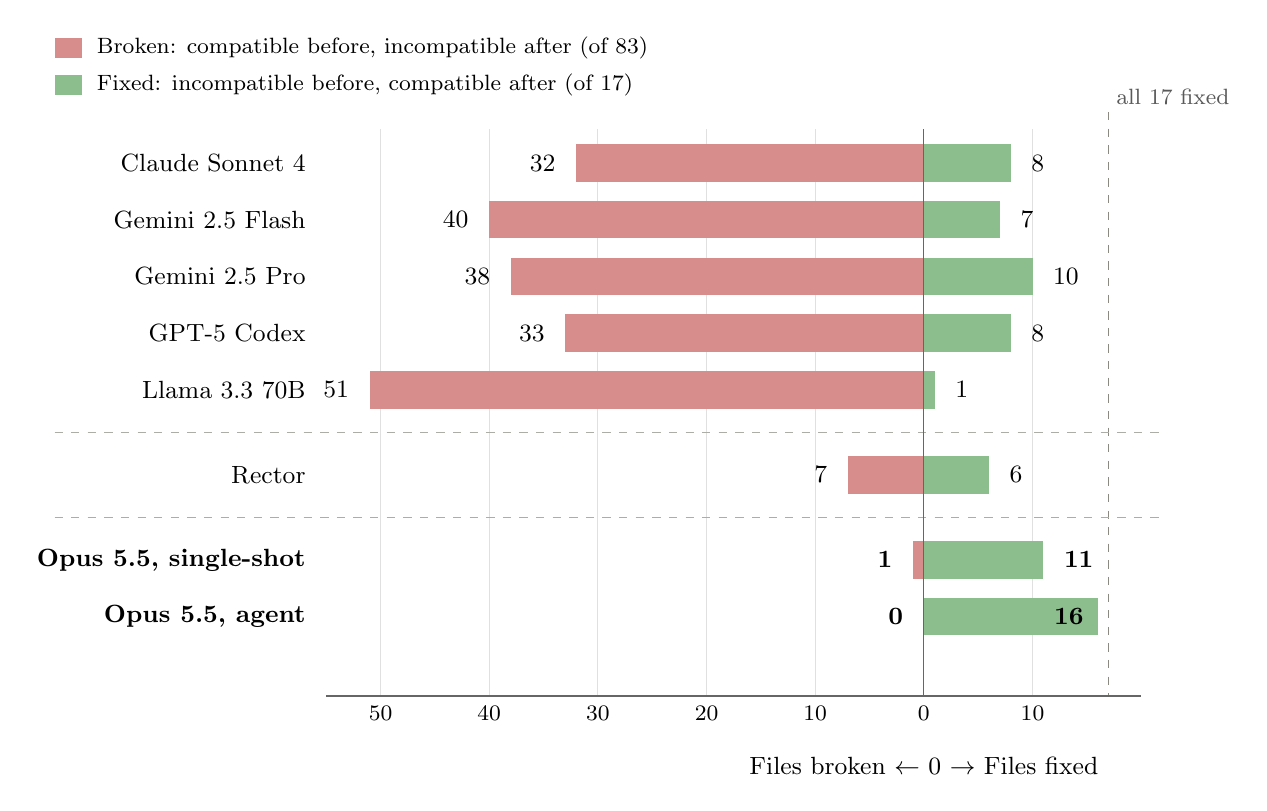
\begin{tikzpicture}[font=\small,x=1.38mm,y=-7.2mm]
  % rows: name / broken / fixed / mine
  \def\rows{{"Claude Sonnet 4",32,8,0},{"Gemini 2.5 Flash",40,7,0},{"Gemini 2.5 Pro",38,10,0},{"GPT-5 Codex",33,8,0},{"Llama 3.3 70B",51,1,0}}
  \foreach \t in {-50,-40,-30,-20,-10,0,10} {\draw[black!12] (\t,-0.6) -- (\t,9.4);}
  \draw[edge,dashed] (17,-0.9) -- (17,9.4) node[pos=0,above right=-1pt,font=\footnotesize,text=black!65] {all 17 fixed};
  \foreach \n/\b/\f/\y in {Claude Sonnet 4/32/8/0, Gemini 2.5 Flash/40/7/1, Gemini 2.5 Pro/38/10/2, GPT-5 Codex/33/8/3, Llama 3.3 70B/51/1/4, Rector/7/6/5.5} {
    \fill[broken!65] (-\b,\y-0.33) rectangle (0,\y+0.33);
    \fill[fixed!65] (0,\y-0.33) rectangle (\f,\y+0.33);
    \node[anchor=east] at (-\b-1,\y) {\b};
    \node[anchor=west] at (\f+1,\y) {\f};
    \node[anchor=east] at (-56,\y) {\n};
  }
  \foreach \n/\b/\f/\y in {Opus 5.5{,} single-shot/1/11/7, Opus 5.5{,} agent/0/16/8} {
    \fill[broken!65] (-\b,\y-0.33) rectangle (0,\y+0.33);
    \fill[fixed!65] (0,\y-0.33) rectangle (\f,\y+0.33);
    \node[anchor=east,font=\small\bfseries] at (-\b-1,\y) {\b};
    \node[anchor=east,font=\small\bfseries] at (-56,\y) {\n};
  }
  \node[anchor=west,font=\small\bfseries] at (12,7) {11};
  \node[anchor=east,font=\small\bfseries] at (15.6,8) {16};
  \draw[edge!70,dashed] (-80,4.75) -- (22,4.75);
  \draw[edge!70,dashed] (-80,6.25) -- (22,6.25);
  \draw[black!60] (0,-0.6) -- (0,9.4);
  \draw[black!60] (-55,9.4) -- (20,9.4);
  \foreach \t in {-50,-40,-30,-20,-10,0,10} {\pgfmathtruncatemacro\a{abs(\t)}\node[below,font=\footnotesize] at (\t,9.4) {\a};}
  \node[below] at (0,10.3) {Files broken $\leftarrow$ 0 $\rightarrow$ Files fixed};
  \fill[broken!65] (-80,-2.2) rectangle (-77.5,-1.85); \node[anchor=west,font=\footnotesize] at (-77,-2.03) {Broken: compatible before, incompatible after (of 83)};
  \fill[fixed!65] (-80,-1.55) rectangle (-77.5,-1.2); \node[anchor=west,font=\footnotesize] at (-77,-1.38) {Fixed: incompatible before, compatible after (of 17)};
\end{tikzpicture}
\caption{Files broken and fixed per approach. The top five rows are the models of~\cite{mahmud2026modernization}, then Rector, then our two conditions (single-shot strict; as delivered it fixes 12). Rows from~\cite{mahmud2026modernization} are recomputed from the package's \code{per\_file.csv} and match the paper's figure; Opus rows come from \code{runs/*/score/per\_file.csv}.}
\label{fig:brokenfixed}
\end{figure}

\subsection{RQ2: The model alone exceeds the unchanged code}

With the study's prompt, limits, and no feedback, Opus 5.5 produces 93 compatible files (94 as delivered).
That is 10 more than the unchanged code, 11 more than Rector, and 34 more than the best model in~\cite{mahmud2026modernization}; it is also 24 more than the best lint-fallback result of that study (GPT-5 Codex, 69).
It breaks one check across 531 original passes, a semantic-fingerprint check for nav-menu sorting in file 054, and repairs 81 of the 99 failing checks (87 as delivered).
Of the 99 responses within the study's limits, all were complete on the first attempt.

The strict single-shot result fails checks in 7 files.
Apart from 009 (Section~\ref{sec:009}) and the over-limit 014, the failures are narrow: 3 of 7 checks for \code{class-wp.php} request parsing (007), one AC3 lookup table (016), POP3's empty-mailbox marker (021), JSON encoding of primitives (030), and the nav-menu regression (054).
On legacy patterns, single-shot Opus 5.5 resolves 66.3\% of findings (67.5\% as delivered) and introduces 26.
That is more than Sonnet 4 and GPT-5 Codex and less than Gemini 2.5 Pro (72.8\%).
Only 21 files leave both all checks passing and no Rector findings.

\subsection{RQ3: With tools and the checks, the migration is behavior-preserving}
\label{sec:rq3}

As an agent, Opus 5.5 breaks none of the 531 passing checks and repairs 93 of 99 failing ones.
All 6 unrepaired checks belong to file 009.
It passes every file the single-shot run left failing except 009 and raises resolution from 66.3\% to 92.4\%, introducing 4 new findings.
Altogether 68 files finish with all checks passing and no remaining Rector findings.

The agent's instructions allow a finding to stay when applying it would change behavior or call compatibility.
Of the 511 original findings, 39 remain, and the agent introduced 4 new ones.
The resulting 43 findings fall under 10 rules, most of them optional rewrites (Figure~\ref{fig:remaining}).
The agent's definition of done asked for no remaining Rector findings unless keeping one was justified.
That instruction targets the aggregate resolution metric that~\cite{mahmud2026modernization} argues is misleading, so we read the agent's resolution together with the necessity breakdown in Section~\ref{sec:necessity} rather than on its own.

\begin{figure}[t]
\centering
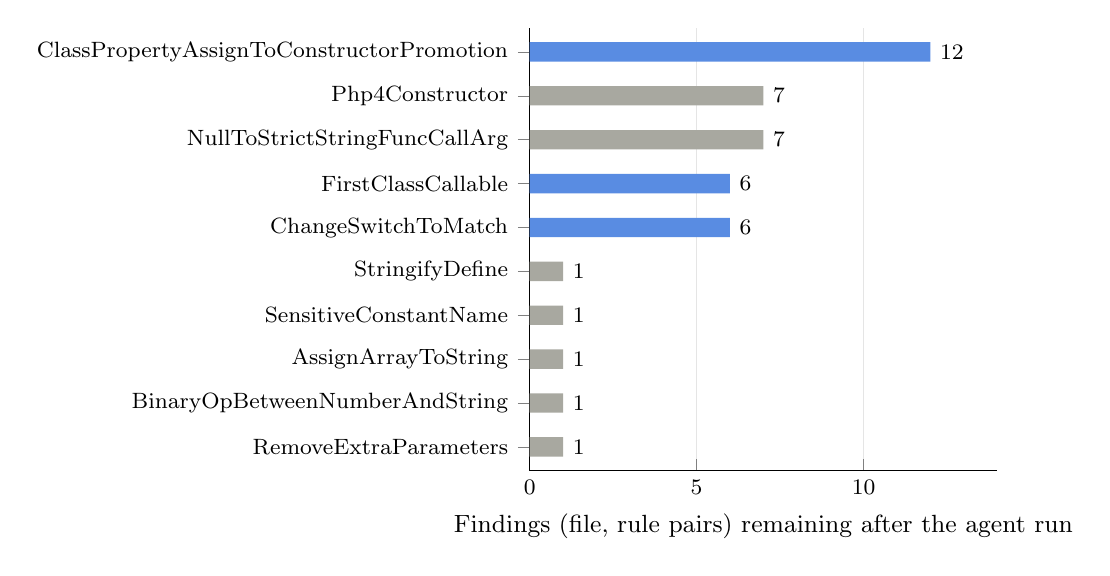
\begin{tikzpicture}
\begin{axis}[xbar, width=0.62\linewidth, height=72mm, bar width=7pt,
  y dir=reverse, bar shift=0pt, enlarge y limits=0.06, ytick={ClassPropertyAssignToConstructorPromotion,Php4Constructor,NullToStrictStringFuncCallArg,FirstClassCallable,ChangeSwitchToMatch,StringifyDefine,SensitiveConstantName,AssignArrayToString,BinaryOpBetweenNumberAndString,RemoveExtraParameters}, xmin=0, xmax=14,
  symbolic y coords={ClassPropertyAssignToConstructorPromotion,Php4Constructor,NullToStrictStringFuncCallArg,FirstClassCallable,ChangeSwitchToMatch,StringifyDefine,SensitiveConstantName,AssignArrayToString,BinaryOpBetweenNumberAndString,RemoveExtraParameters},
  yticklabel style={font=\footnotesize}, xticklabel style={font=\footnotesize},
  axis x line*=bottom, axis y line*=left, xmajorgrids, grid style={black!10},
  nodes near coords, nodes near coords style={font=\footnotesize},
  xlabel={Findings (file, rule pairs) remaining after the agent run}, xlabel style={font=\small}]
\addplot[fill=accent!80,draw=none] coordinates {(12,ClassPropertyAssignToConstructorPromotion) (6,FirstClassCallable) (6,ChangeSwitchToMatch)};
\addplot[fill=muted,draw=none] coordinates {(7,Php4Constructor) (7,NullToStrictStringFuncCallArg) (1,StringifyDefine) (1,SensitiveConstantName) (1,AssignArrayToString) (1,BinaryOpBetweenNumberAndString) (1,RemoveExtraParameters)};
\end{axis}
\end{tikzpicture}
\caption{Rector \code{Php*} findings, as (file, rule) pairs, in the agent run's 100 migrated files, by rule: 43 findings across 10 rules, of which 24 are optional rewrites (blue). Grey: old-style constructors kept as compatibility wrappers (\code{Php4Constructor}), casts on request values (\code{NullToStrict}), and single cases. Source: \code{runs/opus55/score/per\_file.csv}.}
\label{fig:remaining}
\end{figure}

In 30 of the 32 files that keep findings, the agent's final report names every kept rule and gives a reason.
The reports for 010 and 022 name some but not all.
The reasons fall into three groups:
\begin{itemize}
  \item \textbf{Optional modernization.} Constructor promotion, \code{switch} to \code{match}, and first-class callables are valid PHP 8.3 without them and raise no notice. Agents declined them where they would reorder properties visible to \code{get\_object\_vars()}, or where \code{match}'s strict comparison would differ from \code{switch}'s loose one.
  \item \textbf{Compatibility shims.} Seven \code{Php4ConstructorRector} findings remain where the agent added \code{\_\_construct} but kept the old same-name constructor as a forwarding wrapper. WordPress subclasses such as \code{wp\_xmlrpc\_server} still call \code{\$this->IXR\_Server(...)}.
  \item \textbf{Defensive casts.} The agents declined \code{NullToStrictStringFuncCallArgRector} casts on request superglobals whose values are always strings at runtime.
\end{itemize}

In all 100 retained workspaces, no file outside the target differs from the pristine harness, including the WordPress tree, \code{vendor/}, and \code{phpunit.xml} (\code{runs/opus55/tamper\_full.txt}).
All 100 sessions hit at least one permission denial, 123 in total.
All but one were compound shell commands (chained with \code{\&\&} or \code{;}, piped, or using heredocs or redirects), which the per-command allowlist does not match; 52 of them were in-place \code{perl} edits.
Despite the denials, every session ended with a migrated file and a final report.

\paragraph{Cost and effort.}
The agent run cost \$39.66 in total: a median of \$0.30, 14 turns, and 73\,s per file, with at most \$1.56, 59 turns, and 359\,s.
The single-shot run cost \$26.92, a median of \$0.19 per file.
After the single pilot session on file 004, the batch of the other 99 sessions took about 30 minutes of wall-clock time at six sessions in parallel.

\subsection{Necessity, sensitivity, and significance}
\label{sec:necessity}

The original package does not include the rule-to-necessity mapping that~\cite{mahmud2026modernization} uses (its source notes the mapping as incomplete), so we reconstructed one from the study's definitions.
Thirteen rules are \emph{required}, among them curly-brace offsets, PHP 4 constructors, \code{ereg}, \code{create\_function}, \code{each}, case-insensitive constants, and integer needles.
Three are \emph{deprecated}: null-to-string arguments, \code{utf8\_encode}/\code{decode}, and \code{final private}.
The rest are optional.
The mapping reproduces the published group sizes, all 15 of the study's per-model resolution rates, and its five introduced counts (Table~\ref{tab:repro}); it is in \code{runs/reanalysis/necessity\_mapping.csv}.
Table~\ref{tab:necessity} applies it, together with the study's sensitivity analyses and tests, to both Opus conditions.

\begin{table}[t]
\centering\small
\caption{Resolution by necessity, the file split by whether a file contains a required finding, and the two sensitivity analyses of~\cite{mahmud2026modernization}. Rows above the rule are computed by our script and reproduce that study's Tables III and IV; Rector's resolution is not scored. Broken counts come from the 10 compatible files with a required finding and the 73 without; fixed counts from the 16 incompatible files with one. Source: \code{runs/reanalysis/summary.json}.}
\label{tab:necessity}
\setlength{\tabcolsep}{3.5pt}\begin{tabular}{lrrrrcrr}
\toprule
& \multicolumn{3}{c}{Resolution (\%)} & \multicolumn{2}{c}{Files broken / fixed} & \multicolumn{2}{c}{Compatible files} \\
\cmidrule(lr){2-4}\cmidrule(lr){5-6}\cmidrule(lr){7-8}
Approach & \shortstack{Req.\\(37)} & \shortstack{Depr.\\(85)} & \shortstack{Opt.\\(389)} & \shortstack{no req.\\broken} & \shortstack{req.\\broken / fixed} & \shortstack{No\\FP} & \shortstack{Lint\\fallback} \\
\midrule
Claude Sonnet 4 & 78.4 & 8.2 & 60.7 & 26 & 6 / 7 & 62 & 67 \\
Gemini 2.5 Flash & 78.4 & 22.4 & 57.8 & 33 & 7 / 6 & 53 & 65 \\
Gemini 2.5 Pro & 78.4 & 22.4 & 83.3 & 32 & 6 / 9 & 56 & 64 \\
GPT-5 Codex & 56.8 & 32.9 & 63.8 & 28 & 5 / 7 & 60 & 69 \\
Llama 3.3 70B & 45.9 & 9.4 & 33.7 & 44 & 7 / 1 & 36 & 45 \\
Rector & -- & -- & -- & 6 & 1 / 6 & 82 & 82 \\
\midrule
Opus 5.5, single-shot (strict) & 59.5 & 44.7 & 71.7 & 1 & 0 / 10 & 94 & 93 \\
\quad as delivered & 62.2 & 45.9 & 72.8 & 1 & 0 / 11 & 95 & 94 \\
Opus 5.5, agent & 75.7 & 91.8 & 94.1 & 0 & 0 / 15 & 99 & 99 \\
\bottomrule
\end{tabular}
\end{table}

\paragraph{The original's central finding does not recur.}
The study's models break 26--44 of the 73 compatible files that need no required change.
Single-shot Opus 5.5 breaks one of them (054), and the agent breaks none.
Neither Opus condition breaks a compatible file that contains a required finding.
Optional changes still dominate what Opus resolves (82.3\% of resolved findings single-shot, 77.5\% for the agent), but unlike the earlier models' optional changes, they rarely cost behavior.

\paragraph{Required findings.}
On required findings the agent resolves 75.7\%, slightly below the 78.4\% of Sonnet 4 and both Gemini models, although every file in which one still fires passes its checks.
Of the nine that still fire, five are PHP 4 constructors where the agent added \code{\_\_construct} and kept the old name as a forwarding wrapper, so the rule still matches the wrapper.
The other four the agent's reports describe as false positives or as fixed at the failing site.
In 002, applying \code{SensitiveConstantNameRector} would rename constants that the file defines with mixed case.
In 005, the agent made \code{\$this->results[] = \ldots} safe where it occurs rather than changing a public default the checks read.
In 066, subclasses use the argument that \code{RemoveExtraParametersRector} would drop.
Single-shot resolves 59.5\% of required findings, below the study's three strongest models, yet it fixes 10 of the 16 files with a required finding.
Resolution by rule type and compatibility measure different things here, as~\cite{mahmud2026modernization} argues.

\paragraph{Sensitivity.}
Neither Opus condition has a lint failure, so the lint fallback changes nothing.
Without fingerprint checks the strict single-shot result rises to 94, because its only regression (054) is a fingerprint check.
The best result of any earlier model under either analysis is 69.

\paragraph{Significance.}
We apply the study's tests to 11 comparisons of our choosing and correct them jointly with Holm--Bonferroni; this family differs from the study's 21 pairwise comparisons among its own approaches.
Both Opus conditions have significantly more compatible files than the unchanged code.
For the strict single-shot condition the counts are 11 files gained and 1 lost, a difference of $+10$ with 95\% CI $[4, 17]$ and adjusted $p = 0.025$.
For the agent they are 16 and 0, a difference of $+16$ with CI $[9, 23]$ and $p = 2\times10^{-4}$.
Both also exceed Sonnet 4 and Rector (adjusted $p \le 0.025$).
The agent's advantage over single-shot (6 files to 0 strict, 5 to 0 as delivered) has a bootstrap interval above zero ($[2, 11]$) but is not significant under the exact test after correction (adjusted $p = 0.062$; unadjusted 0.031 strict, 0.062 as delivered).
On this single run, then, the agent's gain over single-shot is suggestive, not established.

\subsection{File 009 is blocked by its test environment}
\label{sec:009}

Every approach in Table~\ref{tab:main} scores 0 of 6 on \code{getid3.php} (009).
Its checks construct a \code{getID3} object, whose constructor \code{include}s \code{getid3.lib.php} from the sandboxed WordPress tree.
That library is a separate subject (001), but the harness gives each subject an unmigrated copy of the WordPress 4.0 tree, and the 4.0 library still uses curly-brace string offsets, which PHP 8 rejects at compile time.
The test file defines a \code{getid3\_lib} stub for this purpose, but it writes the stub only if the library file is absent, and the sandbox always contains the real file, so the stub never takes effect.
That is a defect in the harness, not in the migrations.
An edit to \code{getid3.php} could still pass the checks by changing how it loads its own library.
The 009 agent named that option, declined it as gaming the tests, and reported the stub-ordering problem instead.
Excluding 009, the agent condition passes every check on all 99 remaining files.

\section{Discussion}

\paragraph{Model and harness contribute different things.}
Holding the protocol fixed, changing the model, together with its default thinking and sampling settings and the CLI's system prompt, moves compatible files from 59 to 93 and regressions from 126 to 1.
Holding the model fixed, adding the tool loop moves compatible files from 93 to 99 and Rector resolution from 66.3\% to 92.4\%; on one run the file-level gain is not significant (Section~\ref{sec:necessity}).
Most of the behavioral gap reported in~\cite{mahmud2026modernization} therefore closes with a newer model under the same protocol.
Part of that improvement could come from exposure to later, already-modernized WordPress releases; Section~\ref{sec:threats} reports a check that finds little verbatim reuse but cannot rule it out.
Prior work found the same split between generating and executing.
In self-debugging~\cite{chen2024selfdebug}, execution feedback added about 12 points on translation and explanation without execution about 3.5.
In SWE-agent~\cite{yang2024sweagent}, the same model resolved roughly seven times more issues once it could act on a repository.
The agent loop contributes the long tail of behavioral fixes and most of the gain in resolution, chiefly of deprecated findings (44.7\% to 91.8\%) and optional ones (71.7\% to 94.1\%).
A single-shot model leaves about a third of the legacy patterns in place, while the agent removes most of them and explains the rest.

\paragraph{The agent outperforms Rector on preservation and repair.}
Rector is the safest single-shot option in~\cite{mahmud2026modernization}: 97.7\% preservation, because its rewrites are mechanical.
Its 62.6\% repair shows the limit of local rules.
Many legacy failures are semantic, for example \code{count()} on \code{null}, removed functions that need a behavior-equivalent replacement, and \code{htmlspecialchars} defaults that changed in PHP 8.1.
Repairing them requires reasoning about intended behavior.
The agent reaches 100\% preservation and 93.9\% repair, and it uses Rector as a tool.
Rector's diff shows the agent what remains, and the checks tell it which suggested rewrites are unsafe.
Rule-based and LLM-based migration are complements in this workflow, not rivals.
Because~\cite{mahmud2026modernization} does not score Rector's resolution against its own rules, we make no comparison with Rector on modernization.

\begin{figure}[t]
\centering
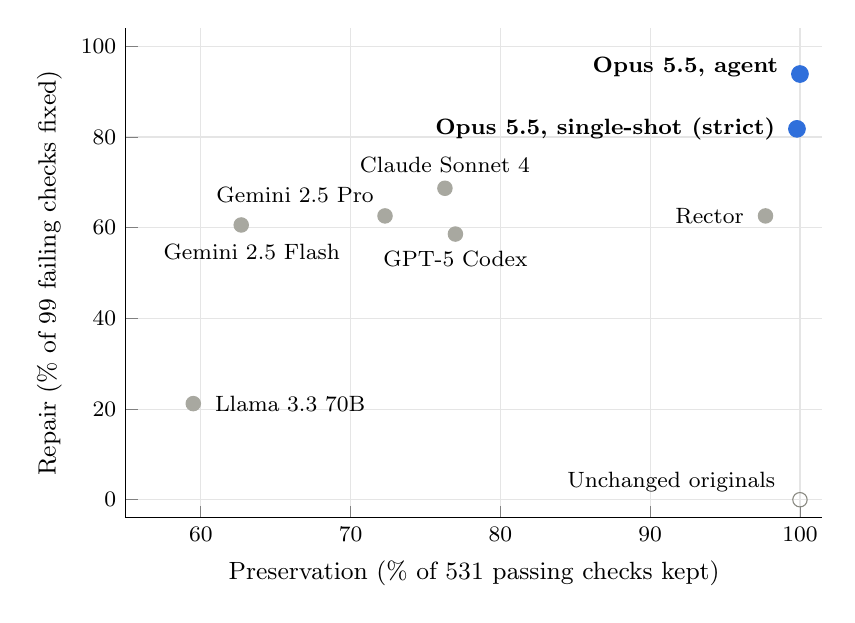
\begin{tikzpicture}
\begin{axis}[width=0.86\linewidth, height=78mm, xmin=55, xmax=101.5, ymin=-4, ymax=104,
  xlabel={Preservation (\% of 531 passing checks kept)}, ylabel={Repair (\% of 99 failing checks fixed)},
  xtick={60,70,80,90,100}, ytick={0,20,40,60,80,100}, grid=major, grid style={black!10},
  tick label style={font=\footnotesize}, label style={font=\small}, axis lines*=left]
  \addplot[only marks, mark=*, mark size=2.6pt, color=muted] coordinates {(59.5,21.2) (62.7,60.6) (72.3,62.6) (77.0,58.6) (76.3,68.7) (97.7,62.6)};
  \addplot[only marks, mark=o, mark size=2.6pt, color=edge] coordinates {(100,0)};
  \addplot[only marks, mark=*, mark size=3pt, color=accent] coordinates {(99.8,81.8) (100,93.9)};
  \node[anchor=west,font=\footnotesize] at (axis cs:60.3,21.2) {Llama 3.3 70B};
  \node[anchor=north,font=\footnotesize] at (axis cs:63.4,58.6) {Gemini 2.5 Flash};
  \node[anchor=south east,font=\footnotesize] at (axis cs:72.2,63.4) {Gemini 2.5 Pro};
  \node[anchor=north,font=\footnotesize] at (axis cs:77.0,57.0) {GPT-5 Codex};
  \node[anchor=south,font=\footnotesize] at (axis cs:76.3,70.0) {Claude Sonnet 4};
  \node[anchor=east,font=\footnotesize] at (axis cs:96.9,62.6) {Rector};
  \node[anchor=east,font=\footnotesize] at (axis cs:99.0,4.0) {Unchanged originals};
  \node[anchor=east,font=\footnotesize\bfseries] at (axis cs:99.0,81.8) {Opus 5.5, single-shot (strict)};
  \node[anchor=east,font=\footnotesize\bfseries] at (axis cs:99.2,95.5) {Opus 5.5, agent};
\end{axis}
\end{tikzpicture}
\caption{Preservation vs.\ repair per approach. The models in~\cite{mahmud2026modernization} trade one rate against the other in the lower left; Rector sits at high preservation but repairs no more than they do; both Opus conditions occupy the corner that neither rules nor older models reach. Rows from~\cite{mahmud2026modernization} are computed from the package's \code{summary.csv}; Opus rows from \code{runs/*/score/summary.json}.}
\label{fig:scatter}
\end{figure}

Figure~\ref{fig:scatter} places each approach by the two rates.
Listing~\ref{lst:ixr} shows two repairs from file 004 (\code{class-IXR.php}) that rules cannot make.
Rector's \code{Php4ConstructorRector} renames \code{IXR\_Server()} to \code{\_\_construct()} and drops the old name.
But WordPress's own \code{wp\_xmlrpc\_server} still calls \code{\$this->IXR\_Server(\$this->methods)} (\code{class-wp-xmlrpc-server.php}, line 159).
In PHP 8 a same-name method no longer acts as a constructor.
Rector's rename restores construction but makes that explicit call fail with an undefined-method error.
Rector also has no rule for \code{count()} on \code{null}, which throws a \code{TypeError} in PHP 8.
According to its final report, the agent found both by reading the callers and running the checks.
That account cannot be verified, because the sessions' turn-by-turn records were not kept.
The wrapper also matches, token for token, the shim WordPress itself has shipped in \code{class-IXR-server.php} since its PHP 4 constructor deprecations, and the single-shot run produced the same ten wrappers.
This example therefore shows a repair that rules miss; it cannot distinguish reasoning from recall.

\begin{lstlisting}[float=t,caption={File 004: original, Rector's rewrite, and the Opus 5.5 agent's output (excerpts).},label={lst:ixr}]
// Original (WordPress 4.0)
function IXR_Server($callbacks = false, $data = false, $wait = false) { ... }
...
if (count($args) == 1) {          // TypeError in PHP 8 when $args is null

// Rector UP_TO_PHP_83: renames the constructor, drops IXR_Server(), leaves count() as is
function __construct($callbacks = false, $data = false, $wait = false) { ... }

// Opus 5.5 agent
public function __construct($callbacks = false, $data = false, $wait = false) { ... }

/**
 * PHP4-style constructor, kept for backward compatibility
 * (e.g. wp_xmlrpc_server calls $this->IXR_Server()).
 */
public function IXR_Server($callbacks = false, $data = false, $wait = false)
{
    self::__construct($callbacks, $data, $wait);
}
...
// (PHP < 8 semantics of count(): null counts as 0, scalars as 1)
$argCount = $args === null ? 0 : (is_countable($args) ? count($args) : 1);
if ($argCount == 1) {
\end{lstlisting}

The kept wrapper is why \code{Php4ConstructorRector} still reports findings after the agent run (Figure~\ref{fig:remaining}).
The agent chose a remaining Rector finding over a broken caller.

\paragraph{Single-shot results are a lower bound.}
The original condition measures how often a model can rewrite a file correctly with no ability to run it.
That is a meaningful quantity: it bounds what a chat-window workflow delivers, and for the models of 2025 it showed they were not reliable when they could not observe behavior.
The study's conclusion is scoped to that condition.
Generalizing it to ``LLMs cannot migrate code'' is not supported by that study, and our results contradict it: under the same protocol for a current model, and with the file's tests for an agent.

\paragraph{Agreement with the original study.}
Our agent condition is, in effect, the staged workflow that~\cite{mahmud2026modernization} recommends in its implications: lint, load with dependencies, check behavior, and let execution feedback drive repair.
Our results confirm that recommendation.
They also support the study's methodological advice: measure against a no-change baseline, report preservation, regressions, and repairs separately, and read resolution by necessity rather than in aggregate.
We add one suggestion: report the model generation and the evaluation condition together, since the same protocol gives opposite headlines for models a year apart.

\paragraph{Harness details matter at this level of performance.}
Once a system passes nearly every check, artifacts in the harness dominate the remaining error.
File 009 accounts for every check the agent fails.
Every approach fails it, because its stub never replaces the unmigrated library it is meant to stand in for.
The Rector metric also depends on running each file in isolation: a directory-level run inflates the original count by 12\%.
Benchmarks for migration should check that each subject is passable under their own protocol, for example by including an oracle migration.

\paragraph{Practical implications.}
At a median of \$0.30 and about a minute per file, an agent loop over an existing test suite is an inexpensive first pass for legacy PHP migration.
Two caveats matter.
The checks here are a sample of each file's contract, so passing them does not prove equivalence, and human review of the diffs remains necessary.
Where no tests exist, an agent can still lint, run Rector, diff behavior against the original on PHP 7, or write its own tests.
Reflexion~\cite{shinn2023reflexion} reached 91\% pass@1 on HumanEval code generation with up to six unit tests that the model generated itself.
That condition is weaker than ours, and we do not measure it.

\section{Threats to Validity}
\label{sec:threats}

\paragraph{Test visibility (construct).}
In the original study the checks are hidden; in our agent condition the model can read and run the same checks that score it.
The agent's 99 files therefore measure what a developer with a test suite achieves, and how well a migration fits a known oracle, not how it generalizes to behavior no test covers.
Its gain over single-shot cannot be attributed to execution feedback in general, as opposed to access to these particular checks.
Several measures limit overfitting: instructions that forbid special-casing and environment detection, scoring against a pristine harness, and the Rector metric, which no test controls.
A search of the agent outputs for test-environment sniffing (\code{phpunit}, the sandbox variables, \code{getenv}) found only an original \code{TMPDIR} lookup in file 015.
These measures do not remove the effect.
A condition with lint, Rector, and PHP but without the checks, or a held-out split of the checks, would separate the two, and we have not run either.
The single-shot condition has no test exposure and still reaches 93 files.

\paragraph{Single run, uncontrolled sampling (conclusion).}
Each condition was run once per file.
The CLI does not expose temperature, so we could not use the study's 0.2, as the study itself could not for GPT-5 Codex.
Results may vary between runs, especially for the single-shot failures.
The margins over the original models (34 or more compatible files, and over 100 fewer regressions) are significant and far larger than plausible run-to-run variation, but the six-file gap between our two conditions is not significant after correction.

\paragraph{Thinking and interface (internal).}
Opus 5.5 used adaptive extended thinking in both conditions.
The client code in~\cite{mahmud2026package} sets no thinking or reasoning parameters, so each model in~\cite{mahmud2026modernization} ran with its provider's default.
For Sonnet 4 that means no extended thinking, while both Gemini 2.5 models think by default~\cite{gemini2026thinking} and GPT-5 Codex is a reasoning model that defaults to medium reasoning effort~\cite{openai2025gpt5codexmodel}.
Our single-shot calls went through the Claude Code CLI with a one-line system prompt, not a raw API call with none.
We consider both part of how the model is used today, but they make the single-shot comparison less than identical.

\paragraph{Environment (internal).}
We used PHP 8.3.36 rather than 8.3.22, and Linux on Apple's Virtualization.framework rather than Windows.
The originals and the archived Sonnet 4 outputs reproduce check for check, and Rector's outputs reproduce its published totals.
For three of the other earlier models the re-score shifts a few checks (at most three per model), plausibly from the PHP patch-level difference, but no compatible-file count changes.
We cannot rule out similar small effects on the new outputs.

\paragraph{Metrics (construct).}
Hidden checks are a sample of each file's contract.
Rector \code{Php*} findings are a proxy for modernization that rewards optional style changes.
A low resolution rate can reflect a deliberate choice not to change behavior, as Section~\ref{sec:rq3} shows, and aggregate resolution mixes required with optional changes (Section~\ref{sec:necessity}).
The necessity mapping is our reconstruction; it reproduces every published rate, but a few rules that fire only once could arguably be grouped differently.

\paragraph{Training-data contamination (internal).}
Later WordPress releases contain PHP 7- and 8-compatible versions of many of these files, and a newer model has likely seen more of them.
That could explain part of the single-shot improvement.
We compared each output's added lines with the same files in WordPress 4.9.35, 6.8.12, and 7.1.4 (\code{harness/contamination.py}).
The metric is the share of non-trivial added lines, compared without whitespace, that appear verbatim in the later file but not in the original.
Rector, which applies fixed rules and cannot be contaminated, gives the chance rate.
Against 7.1.4 the agent's rate is 9.0\% (Rector 7.3\%), single-shot Opus 21.7\%, and Sonnet 4 17.6\%.
Excluding lines that differ from the original only in visibility keywords or braces, the rates are 7.4\%, 6.6\%, 10.9\%, and 9.9\%.
Most single-shot matches reproduce WordPress's coding-standard layout, and the excess largely disappears when only runs of whitespace are collapsed (6.9\% against Rector's 5.7\%).
Every approach's output is less similar to the later file than the original is.
The matching lines are mostly forced PHP 8 fixes and common idioms (\code{??}, \code{\_\_DIR\_\_}, \code{str\_contains}, constructor shims), and no file reuses non-trivial upstream logic.
Line matching cannot separate recall from convergence, and the other LLMs share some of Opus's exposure, so this bounds verbatim reuse but does not rule out contamination.

\paragraph{Protocol deviations (internal).}
Section~\ref{sec:runs} lists every deviation and re-launch.
The single-shot response for file 014 exceeded the study's limits, and our primary result counts it as failed.
In 85 agent prompts the WordPress path was blank, so the agent condition was not uniform in that respect.
Agent 004 was a pilot run before the batch; it used the same prompt template and is the source of Listing~\ref{lst:ixr}.
Re-running the agent condition in one batch with the prompt fixed, and with full session recording, would remove these caveats.

\paragraph{Generalization (external).}
The 100 files are a purposive sample from one application at one version, as~\cite{mahmud2026modernization} notes.
We inherit that limit and add one model from one vendor.

\paragraph{Agent process not recorded (internal).}
The agent runs used Claude Code's headless JSON output, which records each session's final report and statistics (turns, tokens, cost, permission denials) but not the turn-by-turn conversation.
Statements about how an agent reached a result therefore rest on its own final report.
The results themselves do not: every outcome is verified independently by scoring the submitted file.

\paragraph{Evaluator independence.}
The agent harness, prompts, and analysis were built with the help of a Claude-based coding assistant, from the same vendor as the model evaluated.
The scoring code is the original study's harness, and all outputs, final reports, and run statistics are released for inspection.

\section{Conclusion}

The study we revisit found that five 2025-era LLMs, asked once per file and without feedback, left legacy PHP less working than they found it, and it scoped that finding carefully.
The popular reading of that study, that LLMs leave legacy code less working than they found it, does not hold for a current model under the same protocol, and does not hold at all once the model can run its output against the file's tests.
Under the identical single-shot protocol and limits, Claude Opus 5.5 produces 93 compatible files against 83 for the unchanged code, and it breaks only one of the 73 compatible files that need no required change.
As a coding agent with an interpreter, the file's checks, and Rector, the workflow the original study recommends, it produces 99 with no regressions.
Because the agent can read the checks that score it, that figure describes migration with a test suite in hand, not blind generalization.
The remaining file fails because of a defect in its test environment, not the migration.
The question for LLM-based modernization is no longer whether a model can rewrite a file blind, but how to give it the feedback a developer would have, and how to evaluate it under that condition.

\paragraph{Data availability.}
The original replication package is on Zenodo~\cite{mahmud2026package}.
Our package contains the bash port of the runner, the workspace and tool scripts, the agent prompt, the single-shot runner, the scoring and metrics code, each agent session's final report and run statistics, all single-shot responses, the migrated files from both conditions, and per-file and summary scores.
It also contains the re-analysis (\code{harness/reanalysis.py}: necessity mapping, sensitivity analyses, McNemar tests, and bootstrap intervals), the Rector re-score, the full-workspace tamper check, and the contamination check with its per-file results.
It is public at \url{https://github.com/ianiv/php-modernization-agent-replication}.
Local paths in the released records are replaced with \code{<repo>}; the records are otherwise unedited.

\bibliographystyle{unsrtnat}
\bibliography{refs}

\end{document}
